% !TEX encoding = UTF-8 Unicode
\documentclass[10pt]{standalone}\usepackage{tikz}
\usepackage{fontspec}
\setmainfont{Arial}
\setsansfont{Arial}\begin{document}

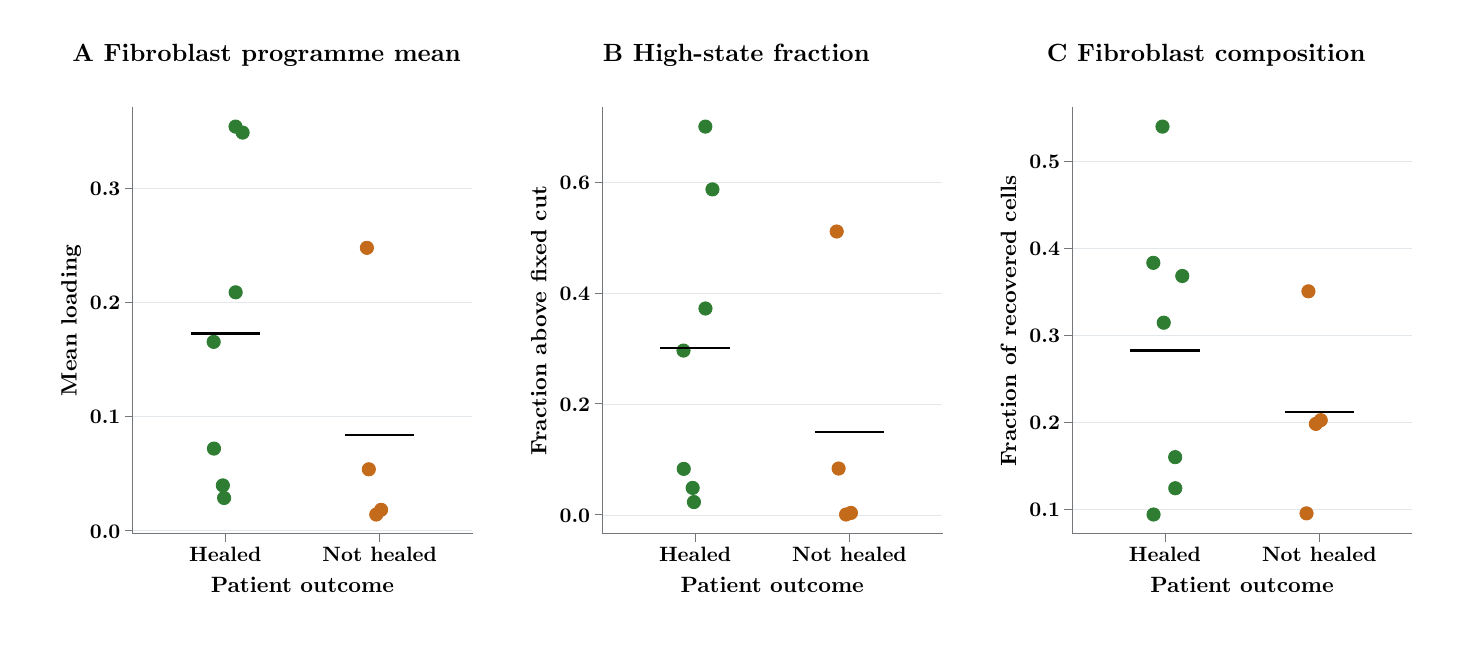
\begin{tikzpicture}[x=1pt,y=1pt]
\definecolor{fillColor}{RGB}{255,255,255}
\path[use as bounding box,fill=fillColor,fill opacity=0.00] (0,0) rectangle (512.15,213.40);
\begin{scope}
\path[clip] (  0.00,  0.00) rectangle (512.15,213.40);
\definecolor{drawColor}{RGB}{0,0,0}

\node[text=drawColor,anchor=base,inner sep=0pt, outer sep=0pt, scale=  0.90] at ( 86.31,201.26) {\bfseries A Fibroblast programme mean};
\end{scope}
\begin{scope}
\path[clip] (  8.54,  4.27) rectangle (164.08,189.78);
\definecolor{fillColor}{RGB}{255,255,255}

\path[fill=fillColor] (  8.54,  4.27) rectangle (164.08,189.78);
\end{scope}
\begin{scope}
\path[clip] ( 37.93, 30.47) rectangle (160.66,184.66);
\definecolor{fillColor}{RGB}{255,255,255}

\path[fill=fillColor] ( 37.93, 30.47) rectangle (160.66,184.66);
\definecolor{drawColor}{RGB}{226,231,235}

\path[draw=drawColor,line width= 0.2pt,line join=round] ( 37.93, 31.62) --
	(160.66, 31.62);

\path[draw=drawColor,line width= 0.2pt,line join=round] ( 37.93, 72.89) --
	(160.66, 72.89);

\path[draw=drawColor,line width= 0.2pt,line join=round] ( 37.93,114.16) --
	(160.66,114.16);

\path[draw=drawColor,line width= 0.2pt,line join=round] ( 37.93,155.43) --
	(160.66,155.43);
\definecolor{drawColor}{RGB}{196,106,27}
\definecolor{fillColor}{RGB}{196,106,27}

\path[draw=drawColor,line width= 0.3pt,line join=round,line cap=round,fill=fillColor] (122.57,133.85) circle (  2.40);
\definecolor{drawColor}{RGB}{46,125,50}
\definecolor{fillColor}{RGB}{46,125,50}

\path[draw=drawColor,line width= 0.3pt,line join=round,line cap=round,fill=fillColor] ( 77.67,175.49) circle (  2.40);

\path[draw=drawColor,line width= 0.3pt,line join=round,line cap=round,fill=fillColor] ( 70.98, 43.46) circle (  2.40);

\path[draw=drawColor,line width= 0.3pt,line join=round,line cap=round,fill=fillColor] ( 75.11,177.65) circle (  2.40);
\definecolor{drawColor}{RGB}{196,106,27}
\definecolor{fillColor}{RGB}{196,106,27}

\path[draw=drawColor,line width= 0.3pt,line join=round,line cap=round,fill=fillColor] (125.96, 37.48) circle (  2.40);

\path[draw=drawColor,line width= 0.3pt,line join=round,line cap=round,fill=fillColor] (127.71, 39.18) circle (  2.40);

\path[draw=drawColor,line width= 0.3pt,line join=round,line cap=round,fill=fillColor] (123.27, 53.82) circle (  2.40);
\definecolor{drawColor}{RGB}{46,125,50}
\definecolor{fillColor}{RGB}{46,125,50}

\path[draw=drawColor,line width= 0.3pt,line join=round,line cap=round,fill=fillColor] ( 67.21, 99.87) circle (  2.40);

\path[draw=drawColor,line width= 0.3pt,line join=round,line cap=round,fill=fillColor] ( 75.15,117.77) circle (  2.40);

\path[draw=drawColor,line width= 0.3pt,line join=round,line cap=round,fill=fillColor] ( 67.31, 61.31) circle (  2.40);

\path[draw=drawColor,line width= 0.3pt,line join=round,line cap=round,fill=fillColor] ( 70.52, 48.00) circle (  2.40);
\definecolor{drawColor}{RGB}{0,0,0}

\path[draw=drawColor,line width= 0.9pt] ( 58.85,102.96) -- ( 83.96,102.96);

\path[draw=drawColor,line width= 0.9pt] (114.64, 66.15) -- (139.74, 66.15);
\end{scope}
\begin{scope}
\path[clip] (  0.00,  0.00) rectangle (512.15,213.40);
\definecolor{drawColor}{RGB}{115,119,123}

\path[draw=drawColor,line width= 0.3pt,line join=round,line cap=rect] ( 37.93, 30.47) --
	( 37.93,184.66);
\end{scope}
\begin{scope}
\path[clip] (  0.00,  0.00) rectangle (512.15,213.40);
\definecolor{drawColor}{RGB}{0,0,0}

\node[text=drawColor,anchor=base east,inner sep=0pt, outer sep=0pt, scale=  0.75] at ( 33.49, 28.93) {\bfseries 0.0};

\node[text=drawColor,anchor=base east,inner sep=0pt, outer sep=0pt, scale=  0.75] at ( 33.49, 70.20) {\bfseries 0.1};

\node[text=drawColor,anchor=base east,inner sep=0pt, outer sep=0pt, scale=  0.75] at ( 33.49,111.47) {\bfseries 0.2};

\node[text=drawColor,anchor=base east,inner sep=0pt, outer sep=0pt, scale=  0.75] at ( 33.49,152.74) {\bfseries 0.3};
\end{scope}
\begin{scope}
\path[clip] (  0.00,  0.00) rectangle (512.15,213.40);
\definecolor{drawColor}{RGB}{115,119,123}

\path[draw=drawColor,line width= 0.3pt,line join=round] ( 35.09, 31.62) --
	( 37.93, 31.62);

\path[draw=drawColor,line width= 0.3pt,line join=round] ( 35.09, 72.89) --
	( 37.93, 72.89);

\path[draw=drawColor,line width= 0.3pt,line join=round] ( 35.09,114.16) --
	( 37.93,114.16);

\path[draw=drawColor,line width= 0.3pt,line join=round] ( 35.09,155.43) --
	( 37.93,155.43);
\end{scope}
\begin{scope}
\path[clip] (  0.00,  0.00) rectangle (512.15,213.40);
\definecolor{drawColor}{RGB}{115,119,123}

\path[draw=drawColor,line width= 0.3pt,line join=round,line cap=rect] ( 37.93, 30.47) --
	(160.66, 30.47);
\end{scope}
\begin{scope}
\path[clip] (  0.00,  0.00) rectangle (512.15,213.40);
\definecolor{drawColor}{RGB}{115,119,123}

\path[draw=drawColor,line width= 0.3pt,line join=round] ( 71.40, 27.62) --
	( 71.40, 30.47);

\path[draw=drawColor,line width= 0.3pt,line join=round] (127.19, 27.62) --
	(127.19, 30.47);
\end{scope}
\begin{scope}
\path[clip] (  0.00,  0.00) rectangle (512.15,213.40);
\definecolor{drawColor}{RGB}{0,0,0}

\node[text=drawColor,anchor=base,inner sep=0pt, outer sep=0pt, scale=  0.75] at ( 71.40, 20.65) {\bfseries Healed};

\node[text=drawColor,anchor=base,inner sep=0pt, outer sep=0pt, scale=  0.75] at (127.19, 20.65) {\bfseries Not healed};
\end{scope}
\begin{scope}
\path[clip] (  0.00,  0.00) rectangle (512.15,213.40);
\definecolor{drawColor}{RGB}{0,0,0}

\node[text=drawColor,anchor=base,inner sep=0pt, outer sep=0pt, scale=  0.80] at ( 99.30,  9.37) {\bfseries Patient outcome};
\end{scope}
\begin{scope}
\path[clip] (  0.00,  0.00) rectangle (512.15,213.40);
\definecolor{drawColor}{RGB}{0,0,0}

\node[text=drawColor,rotate= 90.00,anchor=base,inner sep=0pt, outer sep=0pt, scale=  0.80] at ( 17.68,107.56) {\bfseries Mean loading};
\end{scope}
\begin{scope}
\path[clip] (  0.00,  0.00) rectangle (512.15,213.40);
\definecolor{drawColor}{RGB}{0,0,0}

\node[text=drawColor,anchor=base,inner sep=0pt, outer sep=0pt, scale=  0.90] at (256.07,201.26) {\bfseries B High-state fraction};
\end{scope}
\begin{scope}
\path[clip] (178.30,  4.27) rectangle (333.85,189.78);
\definecolor{fillColor}{RGB}{255,255,255}

\path[fill=fillColor] (178.30,  4.27) rectangle (333.85,189.78);
\end{scope}
\begin{scope}
\path[clip] (207.70, 30.47) rectangle (330.43,184.66);
\definecolor{fillColor}{RGB}{255,255,255}

\path[fill=fillColor] (207.70, 30.47) rectangle (330.43,184.66);
\definecolor{drawColor}{RGB}{226,231,235}

\path[draw=drawColor,line width= 0.2pt,line join=round] (207.70, 37.38) --
	(330.43, 37.38);

\path[draw=drawColor,line width= 0.2pt,line join=round] (207.70, 77.46) --
	(330.43, 77.46);

\path[draw=drawColor,line width= 0.2pt,line join=round] (207.70,117.54) --
	(330.43,117.54);

\path[draw=drawColor,line width= 0.2pt,line join=round] (207.70,157.62) --
	(330.43,157.62);
\definecolor{drawColor}{RGB}{196,106,27}
\definecolor{fillColor}{RGB}{196,106,27}

\path[draw=drawColor,line width= 0.3pt,line join=round,line cap=round,fill=fillColor] (292.34,139.74) circle (  2.40);
\definecolor{drawColor}{RGB}{46,125,50}
\definecolor{fillColor}{RGB}{46,125,50}

\path[draw=drawColor,line width= 0.3pt,line join=round,line cap=round,fill=fillColor] (247.44,154.96) circle (  2.40);

\path[draw=drawColor,line width= 0.3pt,line join=round,line cap=round,fill=fillColor] (240.75, 41.98) circle (  2.40);

\path[draw=drawColor,line width= 0.3pt,line join=round,line cap=round,fill=fillColor] (244.88,177.65) circle (  2.40);
\definecolor{drawColor}{RGB}{196,106,27}
\definecolor{fillColor}{RGB}{196,106,27}

\path[draw=drawColor,line width= 0.3pt,line join=round,line cap=round,fill=fillColor] (295.73, 37.48) circle (  2.40);

\path[draw=drawColor,line width= 0.3pt,line join=round,line cap=round,fill=fillColor] (297.48, 38.05) circle (  2.40);

\path[draw=drawColor,line width= 0.3pt,line join=round,line cap=round,fill=fillColor] (293.03, 54.10) circle (  2.40);
\definecolor{drawColor}{RGB}{46,125,50}
\definecolor{fillColor}{RGB}{46,125,50}

\path[draw=drawColor,line width= 0.3pt,line join=round,line cap=round,fill=fillColor] (236.98, 96.72) circle (  2.40);

\path[draw=drawColor,line width= 0.3pt,line join=round,line cap=round,fill=fillColor] (244.92,111.92) circle (  2.40);

\path[draw=drawColor,line width= 0.3pt,line join=round,line cap=round,fill=fillColor] (237.07, 53.97) circle (  2.40);

\path[draw=drawColor,line width= 0.3pt,line join=round,line cap=round,fill=fillColor] (240.29, 47.09) circle (  2.40);
\definecolor{drawColor}{RGB}{0,0,0}

\path[draw=drawColor,line width= 0.9pt] (228.62, 97.70) -- (253.72, 97.70);

\path[draw=drawColor,line width= 0.9pt] (284.41, 67.35) -- (309.51, 67.35);
\end{scope}
\begin{scope}
\path[clip] (  0.00,  0.00) rectangle (512.15,213.40);
\definecolor{drawColor}{RGB}{115,119,123}

\path[draw=drawColor,line width= 0.3pt,line join=round,line cap=rect] (207.70, 30.47) --
	(207.70,184.66);
\end{scope}
\begin{scope}
\path[clip] (  0.00,  0.00) rectangle (512.15,213.40);
\definecolor{drawColor}{RGB}{0,0,0}

\node[text=drawColor,anchor=base east,inner sep=0pt, outer sep=0pt, scale=  0.75] at (203.25, 34.69) {\bfseries 0.0};

\node[text=drawColor,anchor=base east,inner sep=0pt, outer sep=0pt, scale=  0.75] at (203.25, 74.78) {\bfseries 0.2};

\node[text=drawColor,anchor=base east,inner sep=0pt, outer sep=0pt, scale=  0.75] at (203.25,114.86) {\bfseries 0.4};

\node[text=drawColor,anchor=base east,inner sep=0pt, outer sep=0pt, scale=  0.75] at (203.25,154.94) {\bfseries 0.6};
\end{scope}
\begin{scope}
\path[clip] (  0.00,  0.00) rectangle (512.15,213.40);
\definecolor{drawColor}{RGB}{115,119,123}

\path[draw=drawColor,line width= 0.3pt,line join=round] (204.85, 37.38) --
	(207.70, 37.38);

\path[draw=drawColor,line width= 0.3pt,line join=round] (204.85, 77.46) --
	(207.70, 77.46);

\path[draw=drawColor,line width= 0.3pt,line join=round] (204.85,117.54) --
	(207.70,117.54);

\path[draw=drawColor,line width= 0.3pt,line join=round] (204.85,157.62) --
	(207.70,157.62);
\end{scope}
\begin{scope}
\path[clip] (  0.00,  0.00) rectangle (512.15,213.40);
\definecolor{drawColor}{RGB}{115,119,123}

\path[draw=drawColor,line width= 0.3pt,line join=round,line cap=rect] (207.70, 30.47) --
	(330.43, 30.47);
\end{scope}
\begin{scope}
\path[clip] (  0.00,  0.00) rectangle (512.15,213.40);
\definecolor{drawColor}{RGB}{115,119,123}

\path[draw=drawColor,line width= 0.3pt,line join=round] (241.17, 27.62) --
	(241.17, 30.47);

\path[draw=drawColor,line width= 0.3pt,line join=round] (296.96, 27.62) --
	(296.96, 30.47);
\end{scope}
\begin{scope}
\path[clip] (  0.00,  0.00) rectangle (512.15,213.40);
\definecolor{drawColor}{RGB}{0,0,0}

\node[text=drawColor,anchor=base,inner sep=0pt, outer sep=0pt, scale=  0.75] at (241.17, 20.65) {\bfseries Healed};

\node[text=drawColor,anchor=base,inner sep=0pt, outer sep=0pt, scale=  0.75] at (296.96, 20.65) {\bfseries Not healed};
\end{scope}
\begin{scope}
\path[clip] (  0.00,  0.00) rectangle (512.15,213.40);
\definecolor{drawColor}{RGB}{0,0,0}

\node[text=drawColor,anchor=base,inner sep=0pt, outer sep=0pt, scale=  0.80] at (269.06,  9.37) {\bfseries Patient outcome};
\end{scope}
\begin{scope}
\path[clip] (  0.00,  0.00) rectangle (512.15,213.40);
\definecolor{drawColor}{RGB}{0,0,0}

\node[text=drawColor,rotate= 90.00,anchor=base,inner sep=0pt, outer sep=0pt, scale=  0.80] at (187.44,107.56) {\bfseries Fraction above fixed cut};
\end{scope}
\begin{scope}
\path[clip] (  0.00,  0.00) rectangle (512.15,213.40);
\definecolor{drawColor}{RGB}{0,0,0}

\node[text=drawColor,anchor=base,inner sep=0pt, outer sep=0pt, scale=  0.90] at (425.84,201.26) {\bfseries C Fibroblast composition};
\end{scope}
\begin{scope}
\path[clip] (348.07,  4.27) rectangle (503.61,189.78);
\definecolor{fillColor}{RGB}{255,255,255}

\path[fill=fillColor] (348.07,  4.27) rectangle (503.61,189.78);
\end{scope}
\begin{scope}
\path[clip] (377.47, 30.47) rectangle (500.20,184.66);
\definecolor{fillColor}{RGB}{255,255,255}

\path[fill=fillColor] (377.47, 30.47) rectangle (500.20,184.66);
\definecolor{drawColor}{RGB}{226,231,235}

\path[draw=drawColor,line width= 0.2pt,line join=round] (377.47, 39.41) --
	(500.20, 39.41);

\path[draw=drawColor,line width= 0.2pt,line join=round] (377.47, 70.82) --
	(500.20, 70.82);

\path[draw=drawColor,line width= 0.2pt,line join=round] (377.47,102.23) --
	(500.20,102.23);

\path[draw=drawColor,line width= 0.2pt,line join=round] (377.47,133.64) --
	(500.20,133.64);

\path[draw=drawColor,line width= 0.2pt,line join=round] (377.47,165.05) --
	(500.20,165.05);
\definecolor{drawColor}{RGB}{196,106,27}
\definecolor{fillColor}{RGB}{196,106,27}

\path[draw=drawColor,line width= 0.3pt,line join=round,line cap=round,fill=fillColor] (462.11, 37.89) circle (  2.40);
\definecolor{drawColor}{RGB}{46,125,50}
\definecolor{fillColor}{RGB}{46,125,50}

\path[draw=drawColor,line width= 0.3pt,line join=round,line cap=round,fill=fillColor] (417.21,123.67) circle (  2.40);

\path[draw=drawColor,line width= 0.3pt,line join=round,line cap=round,fill=fillColor] (410.51,106.79) circle (  2.40);

\path[draw=drawColor,line width= 0.3pt,line join=round,line cap=round,fill=fillColor] (414.65, 58.21) circle (  2.40);
\definecolor{drawColor}{RGB}{196,106,27}
\definecolor{fillColor}{RGB}{196,106,27}

\path[draw=drawColor,line width= 0.3pt,line join=round,line cap=round,fill=fillColor] (465.49, 70.22) circle (  2.40);

\path[draw=drawColor,line width= 0.3pt,line join=round,line cap=round,fill=fillColor] (467.25, 71.58) circle (  2.40);

\path[draw=drawColor,line width= 0.3pt,line join=round,line cap=round,fill=fillColor] (462.80,118.13) circle (  2.40);
\definecolor{drawColor}{RGB}{46,125,50}
\definecolor{fillColor}{RGB}{46,125,50}

\path[draw=drawColor,line width= 0.3pt,line join=round,line cap=round,fill=fillColor] (406.75,128.42) circle (  2.40);

\path[draw=drawColor,line width= 0.3pt,line join=round,line cap=round,fill=fillColor] (414.69, 46.97) circle (  2.40);

\path[draw=drawColor,line width= 0.3pt,line join=round,line cap=round,fill=fillColor] (406.84, 37.48) circle (  2.40);

\path[draw=drawColor,line width= 0.3pt,line join=round,line cap=round,fill=fillColor] (410.06,177.65) circle (  2.40);
\definecolor{drawColor}{RGB}{0,0,0}

\path[draw=drawColor,line width= 0.9pt] (398.39, 96.74) -- (423.49, 96.74);

\path[draw=drawColor,line width= 0.9pt] (454.17, 74.51) -- (479.28, 74.51);
\end{scope}
\begin{scope}
\path[clip] (  0.00,  0.00) rectangle (512.15,213.40);
\definecolor{drawColor}{RGB}{115,119,123}

\path[draw=drawColor,line width= 0.3pt,line join=round,line cap=rect] (377.47, 30.47) --
	(377.47,184.66);
\end{scope}
\begin{scope}
\path[clip] (  0.00,  0.00) rectangle (512.15,213.40);
\definecolor{drawColor}{RGB}{0,0,0}

\node[text=drawColor,anchor=base east,inner sep=0pt, outer sep=0pt, scale=  0.75] at (373.02, 36.72) {\bfseries 0.1};

\node[text=drawColor,anchor=base east,inner sep=0pt, outer sep=0pt, scale=  0.75] at (373.02, 68.13) {\bfseries 0.2};

\node[text=drawColor,anchor=base east,inner sep=0pt, outer sep=0pt, scale=  0.75] at (373.02, 99.55) {\bfseries 0.3};

\node[text=drawColor,anchor=base east,inner sep=0pt, outer sep=0pt, scale=  0.75] at (373.02,130.96) {\bfseries 0.4};

\node[text=drawColor,anchor=base east,inner sep=0pt, outer sep=0pt, scale=  0.75] at (373.02,162.37) {\bfseries 0.5};
\end{scope}
\begin{scope}
\path[clip] (  0.00,  0.00) rectangle (512.15,213.40);
\definecolor{drawColor}{RGB}{115,119,123}

\path[draw=drawColor,line width= 0.3pt,line join=round] (374.62, 39.41) --
	(377.47, 39.41);

\path[draw=drawColor,line width= 0.3pt,line join=round] (374.62, 70.82) --
	(377.47, 70.82);

\path[draw=drawColor,line width= 0.3pt,line join=round] (374.62,102.23) --
	(377.47,102.23);

\path[draw=drawColor,line width= 0.3pt,line join=round] (374.62,133.64) --
	(377.47,133.64);

\path[draw=drawColor,line width= 0.3pt,line join=round] (374.62,165.05) --
	(377.47,165.05);
\end{scope}
\begin{scope}
\path[clip] (  0.00,  0.00) rectangle (512.15,213.40);
\definecolor{drawColor}{RGB}{115,119,123}

\path[draw=drawColor,line width= 0.3pt,line join=round,line cap=rect] (377.47, 30.47) --
	(500.20, 30.47);
\end{scope}
\begin{scope}
\path[clip] (  0.00,  0.00) rectangle (512.15,213.40);
\definecolor{drawColor}{RGB}{115,119,123}

\path[draw=drawColor,line width= 0.3pt,line join=round] (410.94, 27.62) --
	(410.94, 30.47);

\path[draw=drawColor,line width= 0.3pt,line join=round] (466.73, 27.62) --
	(466.73, 30.47);
\end{scope}
\begin{scope}
\path[clip] (  0.00,  0.00) rectangle (512.15,213.40);
\definecolor{drawColor}{RGB}{0,0,0}

\node[text=drawColor,anchor=base,inner sep=0pt, outer sep=0pt, scale=  0.75] at (410.94, 20.65) {\bfseries Healed};

\node[text=drawColor,anchor=base,inner sep=0pt, outer sep=0pt, scale=  0.75] at (466.73, 20.65) {\bfseries Not healed};
\end{scope}
\begin{scope}
\path[clip] (  0.00,  0.00) rectangle (512.15,213.40);
\definecolor{drawColor}{RGB}{0,0,0}

\node[text=drawColor,anchor=base,inner sep=0pt, outer sep=0pt, scale=  0.80] at (438.83,  9.37) {\bfseries Patient outcome};
\end{scope}
\begin{scope}
\path[clip] (  0.00,  0.00) rectangle (512.15,213.40);
\definecolor{drawColor}{RGB}{0,0,0}

\node[text=drawColor,rotate= 90.00,anchor=base,inner sep=0pt, outer sep=0pt, scale=  0.80] at (357.21,107.56) {\bfseries Fraction of recovered cells};
\end{scope}
\end{tikzpicture}

\end{document}
